\section{Approach}\label{sec:methodology}

\subsection{Data Collection}
A dataset was created for the Java and the C\# programming language. To gather these, the Github API was used to retrieve the top 1000 most-starred repositories for both languages. The choice to separate these datasets is due to the fact that a sequence to sequence deep learning model was trained, as will be explained in \Cref{subsec:model}. The tokens in the input sequence, the git diff files, must originate from the same distribution of input data. Therefore, the decision was made to train a model per programming language. Also, commit messages can be structured differently per programming language as coding convention vary. Therefore, training a model per language could lead to more accurate git commit message generation.

% Dit is niet waar - de verschillende input is belangrijker
%The choice to separate these datasets is due to the hypothesis that git commit messages can differ per programming language, and therefore training a language model per programming language can lead to more accurate git commit message generation.

For each repository, the most recent commits of the default branch (the \textit{master} branch in most cases) were retrieved. For each commit, the commit message and the raw \textit{git diff} output of the commit and it's parent commit were saved. Commits that did not fulfill the following criteria were ignored:
\begin{itemize}
    \item With more than one parent commit (merge commits).
    \item Without a parent commit (initial commits).
    \item With diffs bigger than 1MB. 
\end{itemize}
Also, all messages and diff were encoded in \textit{UTF-8}. Characters not supported by this encoding are replaced with the unicode replacement character. All commits in the default branch, beginning with the most recent one, were collected until all commits in the branch were considered or until 10K commits were collected for that repository.
This results in a dataset for Java with 610.484 messages with diffs and a dataset for C\# with 1.572.274 messages with diffs.

\subsubsection{Training, Validation and Test Set Splits}
The collected data needs to be divided into three distinct sets that have no overlap. These sets will be used as training, validation or testing data respectively. Also, the collected dataset is rather large in size compared to the dataset that \citeauthor{jiang_automatically_2017} used. Therefore, the decision was made to select a equal amount, 36000 objects, at random from the collected dataset. The splits were then created from this subset of 36000 objects according to a ratio of $0.8$, $0.1$ and $0.1$ for training, validation and testing respectively. This division applies for all dataset that were either collected or preprocessed according to our procedure.

\subsection{Encoder-Decoder Model}\label{subsec:model}
The approach to generate commit message from a \textsc{git diff} file will be the same as \citeauthor{jiang_automatically_2017}, namely with the neural machine translation approach that does sequence to sequence learning. The model that is to be used is from \citeauthor{bahdanau2014neural}, a encoder-decoder model that uses attention to attend to the important parts of the \textit{git diff} sequence $\mathbf{x}$ during the generation of the commit message sequence $\mathbf{y}$. A schematic view is given in \Cref{fig:model}. Each of the components of the model will be discussed more thoroughly in the sections below.

\begin{figure}
    \centering
    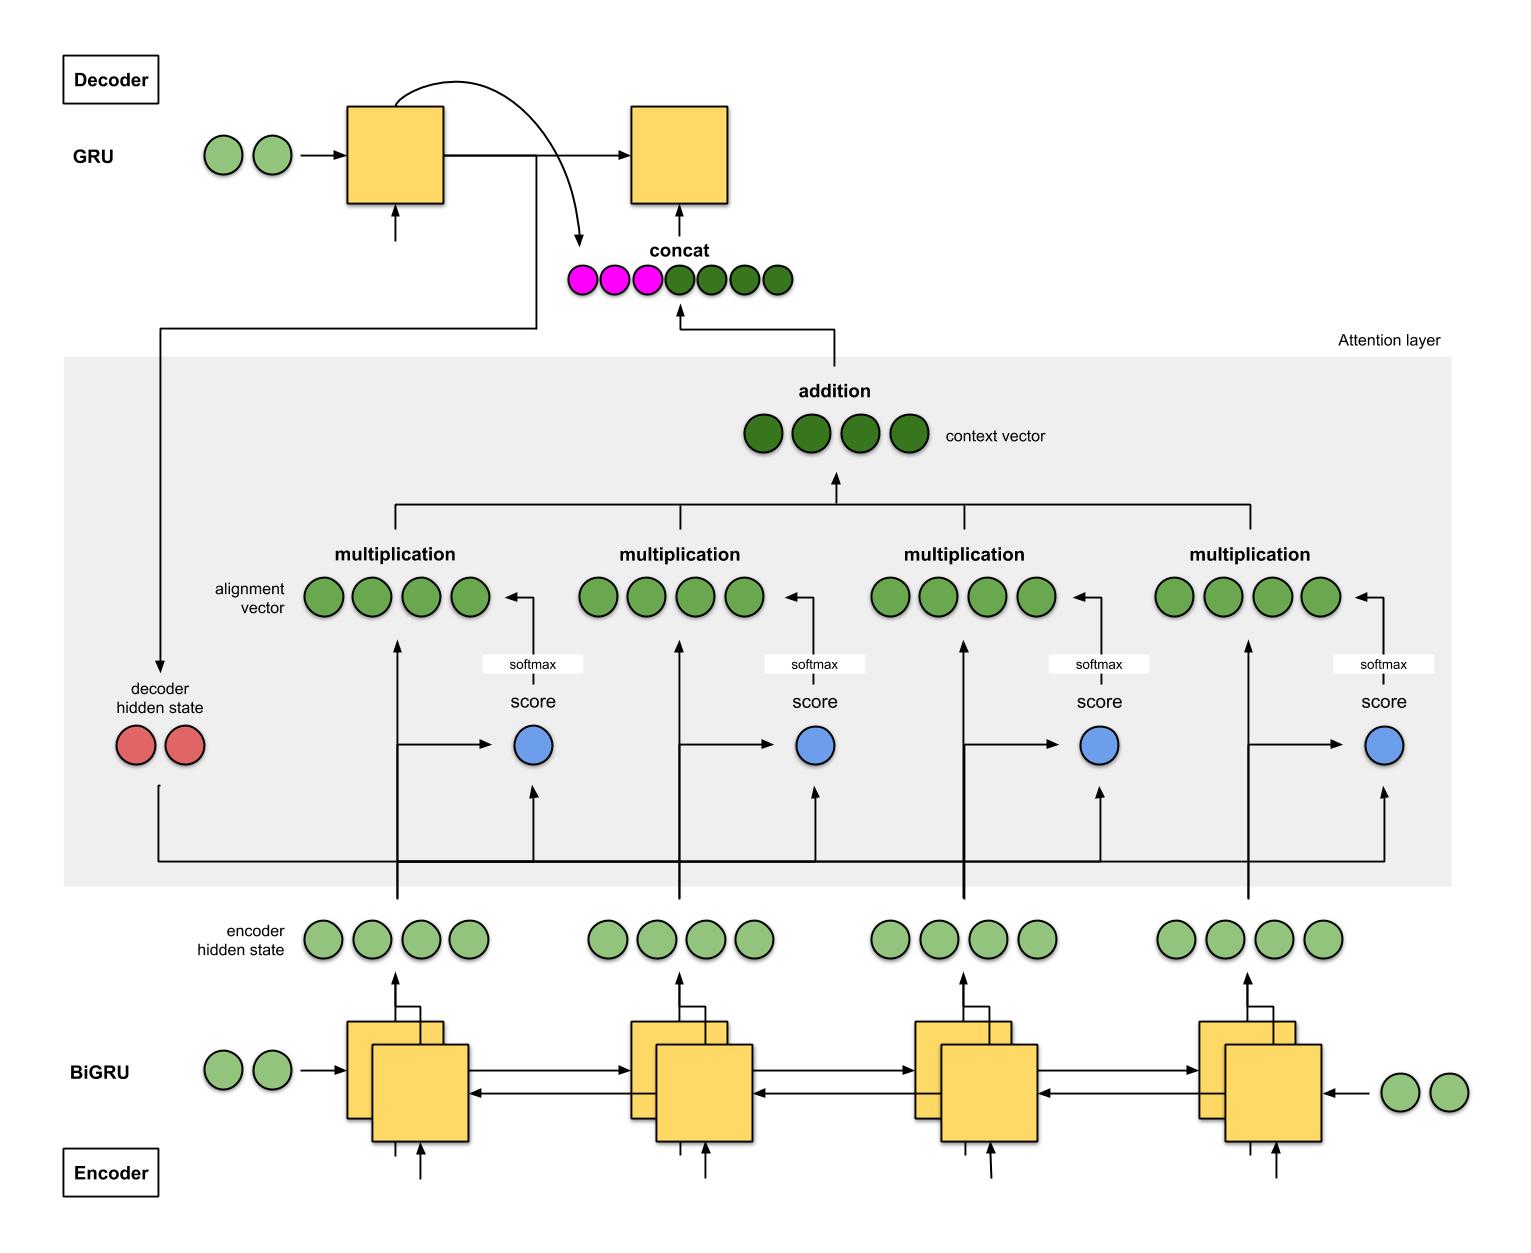
\includegraphics[width=0.5\textwidth]{figs/network.png}
    \caption{The encoder-decoder model that is used for this research. Both the encoder and decoder consist of a GRU, and the encoder is bidirectional. At each time step, a score is computed for each encoder hidden state based on the previous decoder hidden state. This score is changed to a probability (softmax) and multiplied with the corresponding hidden state to yield a context/alignment vector. The input of the decoder for the nex time step is then the sum of these context vectors  and the previous output of the decoder. Image from \cite{network_pic}.}
    \label{fig:model}
\end{figure}

\subsubsection{Encoder}
The encoder processes the variable length source sequence $x = (x_1,...,x_t)$ one token at a time until it reaches the end of the sequence. At each time step $t$, the hidden state $h_t$ is computed as:

$$h_t = f(h_{t-1},x_t)$$

The function $f$ is a non-linear function such as a LSTM or GRU, which both have the same characteristic of providing memory. In this research, the bidirectional GRU was used according to the network of \cite{bahdanau2014neural} that encode the sequence in both a forward manner as $\forward{h_t}$, and backward as $\backward{h_t}$. This means the hidden state at each time step $t$ consists of a concatenation of both states: $h_t= [\forward{h_t},\backward{h_t}$]. Note that each sequence contains a start (\token{sos}) and stop (\token{eos}) symbol, and thus $\forward{x_0} = \token{sos}$ and $\backward{x_0} = \token{eos}$ are the initial input tokens. If all tokens of the sequence are seen by the encoder then the hidden states are passed to the attention layer and decoder. As the decoder is not bidirectional, it initial supplied context vector is computed as:
$$h^{\prime}_0 = f(g(\forward{h_t},\backward{h_t}))$$
where $f$ is the $tanh$ activation function and $g$ is a feedforward layer.

\subsubsection{Decoder}
The decoder processes the provided hidden states $h_t$ from the encoder, and computes a decoder hidden state $h_t^{\prime}$ and the conditional distribution of the target token $y_t$ according to the following equations:

\begin{align*}
h_{t}^{\prime} &= f(h_{t-1}^{\prime}, y_{t-1}, c_{t}) \\
p(y_{t} | y_{t-1}, \ldots, y_{1}, c_{t}) &= g(h_{t}^{\prime}, y_{t-1}, c_{t})
\end{align*}
where $c_{t}$ is the context vector and $f$ and $g$ are both non-linear functions. In this research, $f$ is again a GRU like in the encoder. For the function $g$, it needs to predict probabilities between 0 and 1 and is therefore the $softmax$ function. The context vectors $c_{t}$ are computed by the Attention layer.

\subsubsection{Attention}
The attention used in this model is additive attention according to \citeauthor{bahdanau2014neural}. As the decoder section mentions, the context vectors $c_{t}$ are used in each time step $t$. The context vectors are computed as:
$$
c_{t}=\sum_{i=1}^{T} \alpha_{t i} h_{i}
$$

where the attention $\alpha$ are probabilities that are computed with the $softmax$ function:
$$
\alpha_{i j}=\frac{\exp \left(e_{i j}\right)}{\sum_{k=1}^{T} \exp \left(e_{i k}\right)} = softmax(e_{ij})
$$
The variable $e$ is the \textit{alignment model} score on how well the source ts at index $j$ matches the target at index $i$ match and is computed as:  
$$
e_{i j}=a\left(h^{\prime}_{i-1}, h_{j}\right)
$$
The function $a$ is the \textit{alignment model} and is defined as a feedforward layer in this research and is jointly trained with the total model.

\subsubsection{Embeddings}
A trainable embedding layer $E$ is used in both the encoder and decoder to get numerical representations of the source and target tokens respectively. This matrix consists of $E \in \mathbb{R}^{m \times k}$ where $m$ is the size of the corresponding vocabulary and $k$ is the embedding dimension. A token can now be looked with the one-hot encoding of the token in the vocabulary. Dropout was used after the embedding layers as this leads to a better generalization error in RNN's \cite{gal2016theoretically}.  

\subsubsection{Optimize function}
The goal of the network is to maximize the conditional log-likelihood of the target sequence given the input sequence by adjusting the model parameters:
$$
\max _{\theta} \frac{1}{N} \sum_{i=1}^{N} \log p\left(y_{i} | x_{i} ; \theta\right)
$$
where $N$ is the amount of objects in the dataset, $\theta$ are the parameters of the model, and $x_i$ $y_i$ are tokens from the source and target sequence respectively. In this research, this goal was achieved by minimizing the cross entropy loss, as this gives the same optimal set of parameters $\theta$. 

\subsection{Evaluation}
During training, the model is evaluated on the validation data by computing the cross entropy loss. The model with the lowest loss will be considered the best model. 
During testing, for all models the BLEU scores are computed according to \cite{papineni_bleu:_2001} and the ROUGE F1 scores are computed according to \cite{lin_rouge:_2004}, which is a combination of ROUGE precision and recall. The ROUGE-1 and ROUGE-2 scores are based on the overlap of unigrams and bigrams respectively. ROUGE-L is based on the longest common subsequence (LCS) and ROUGE-W builds further on this by using weighted LCSes which favors consecutive subsequences.

\subsection{Model Training}\label{subsec:training}
Extra techniques were implemented to effectively train a model that performs well. Firstly, teacher forcing is used where with a predefined probability we take the real $y_t$ instead of the predicted $\hat{y_t}$ \cite{williams1989learning}. Secondly, two techniques from NLP are applied: packing and masking. With packing, the length of the source sequence is supplied to the model such that it stops all extra padding tokens are ignored. With masking, a mask is created over all values that are not padding. This mask can then be used to in the computation for attention so that padding tokens are ignored.     

The model was trained with Stochastic Gradient Descent (SGD) with an initial learning rate of $0.1$. The learning rate was reduced with factor $0.1$ if no improvements were made on the validation loss for 10 epochs. Early stopping of the training process was done if no validation loss improvement was seen for 20 epochs. All models were trained on a Nvidia GeForce GTX 1660 GPU with 6GB of memory. After each epoch, the intermediate model was saved and the model with the least validation loss was used for evaluation.
